\documentclass[a4paper,10pt]{article}
\usepackage[utf8]{inputenc}
\usepackage{graphicx}
\begin{document}

\begin{titlepage}
\begin{center}
\vspace*{1.5in}
\begin{Large}
\textbf{Modelos y Simulación}
\vspace{0.5in}

\textbf{Trabajo Especial II}

\vspace{0.3in}
\textbf{Modelo de Inventario}
% \begin{figure}[hbt]
% \noindent\makebox[\textwidth]{
\includegraphics[scale=0.5]{gm}}
% \end{figure}

\vspace{1.5in}
Giovanni Rescia

\vspace*{0.4in}

FaMAF, UNC
\vspace*{.13in}

Junio de 2014
\end{Large}
\end{center}
\end{titlepage}

\author{Giovanni Rescia \\ \\ \large FaMAF}
\date{21 de Mayo de 2014}

\pagebreak

\section*{Resumen}
\vspace{0.4in}
El presente trabajo se desarrollará en el contexto del modelo de inventario dado en el capítulo 6.5 del
libro Simulación de Sheldon M. Ross. El objetivo del mismo es analizar la calidad estadística de una lista
de datos mediante la utilización de diversos test, y no la simulación del mencionado modelo.

Se realizarán test de bondad de ajuste para ver cómo se adaptan distintas distribuciones a los datos listados.

\pagebreak

\section*{Introducción}
\vspace{0.4in}

En particular, trabajaremos con el modelo de inventario bajo las siguiente hipótesis:

\begin{itemize}
 \item El precio del artículo es \$2.
 \item Los clientes aparecen en el sistema según un proceso Poisson con razón 20 por hora.
 \item La cantidad de artículos que cada uno de ellos pide es una variable aleatoria con distribución $\mathcal{G}$(0.4).
 \item El stock mínimo es $s$=5 y el stock máximo es $S$=50. El stock inicial es 50 y es gratis.
 \item El costo de comprar $y$ artículos es una función $c(y)$ = $y + \frac{1}{y}$, y se demoran 5 horas en traerlo.
 \item La tienda paga un costo de mantenimiento del inventario de \$0.10 por cada artículo, por hora cumplida.
 \item El sistema funciona 8hs diarias, 5 días a la semana, reiniciándose al finalizar la semana.
\end{itemize}

\subsection*{Bases teóricas para la resolución del problema}
\vspace{0.4in}
\subsubsection*{Test de Kolmogorov-Smirnov}
El test de Kolmogorov-Smirnov, entre otras cosas, puede ser usado para comparar una muestra bajo la hipótesis que esa
muestra tiene cierta distribución de probabilidad con ciertos parámetros (la llameremos la hipótesis nula, denotada $H_0$).

El resultado de tal pruba es un valor (llamado p-valor), que: o bien nos permite refutar $H_0$, o bien nos dice que
no hay evidencia suficiente para rechazarla.


\subsubsection*{Test $\chi^2$}
Va a ser usado con el mismo propósito que el test de Kolmogorov-Smirnov, solo que para distribuciones discretas (en contraste
con Kolmogorov-Smirnov que es para distribuciones continuas).

\pagebreak

\section*{Independencia de los datos}


A tal fin de observar cuán independientes son los datos muestreados, nos valeremos de un $scatter \ diagram$.
Mientras más dispersos se observen los datos en el gráfico, más independientes serán unos de otros.


\begin{figure}[hbt]
\noindent\makebox[\textwidth]{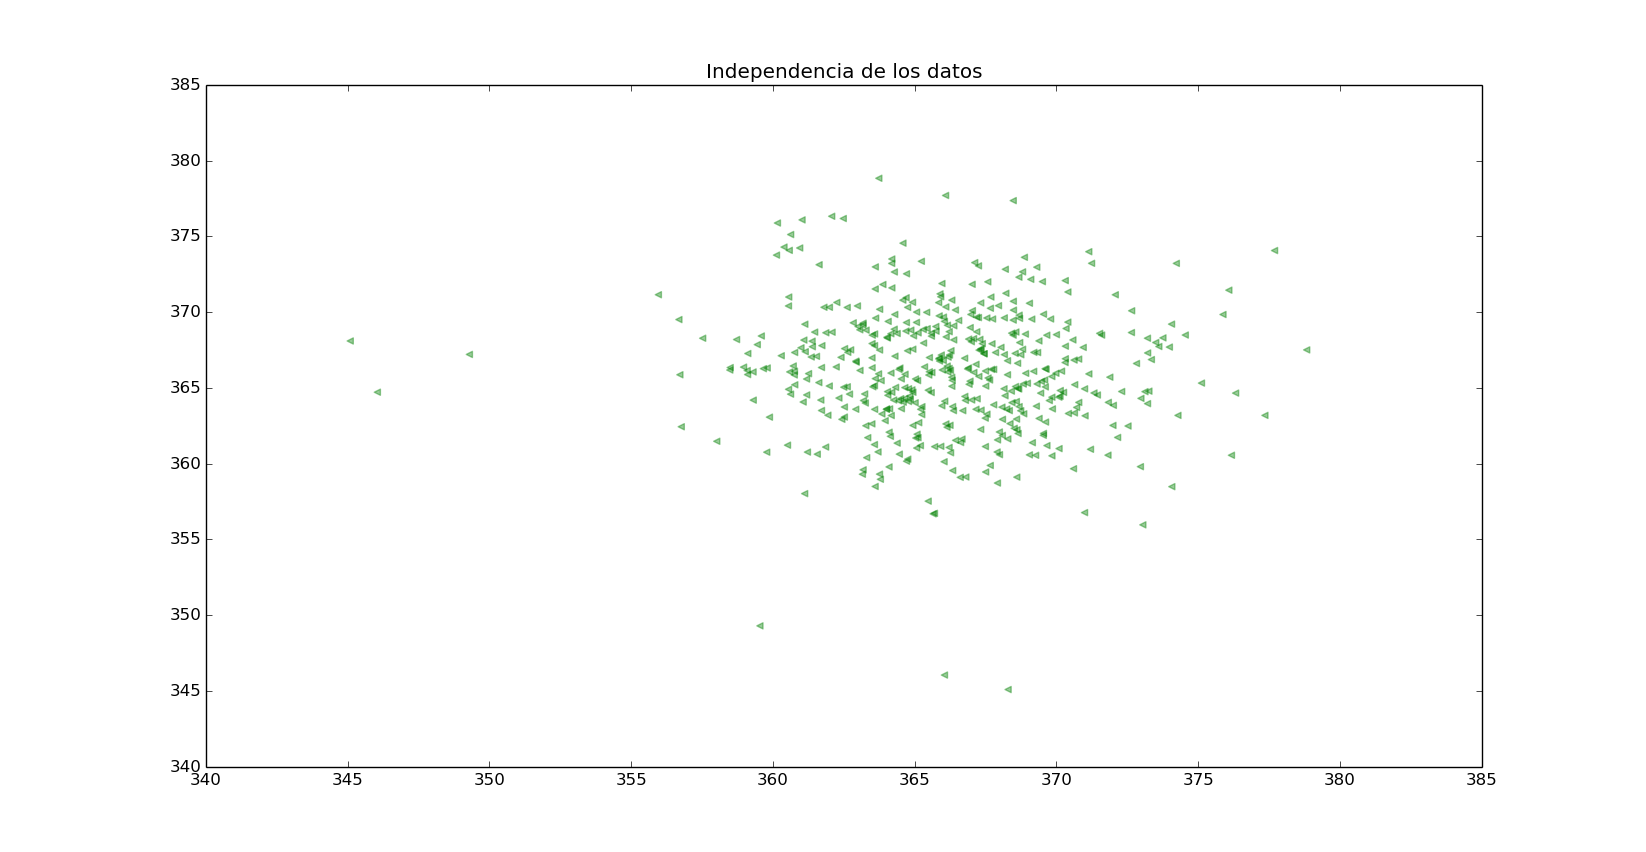
\includegraphics[scale=0.35]{scatter}}
\end{figure}

Como se puede apreciar en el gráfico, los puntos están dispersos, lo que indica independencia.
Otra observación que se puede hacer que es que hay alta concentración de puntos en 366, por lo que la media
se encuentra cerca de 366.

\pagebreak

\section*{Muestras de Variables Aleatorias Geométricas}

A continuación histogramas con 100, 1000 y 10000 variables aleatorias $\sim \mathcal{G}$(0.4).


\begin{figure}[hbt]
\noindent\makebox[\textwidth]{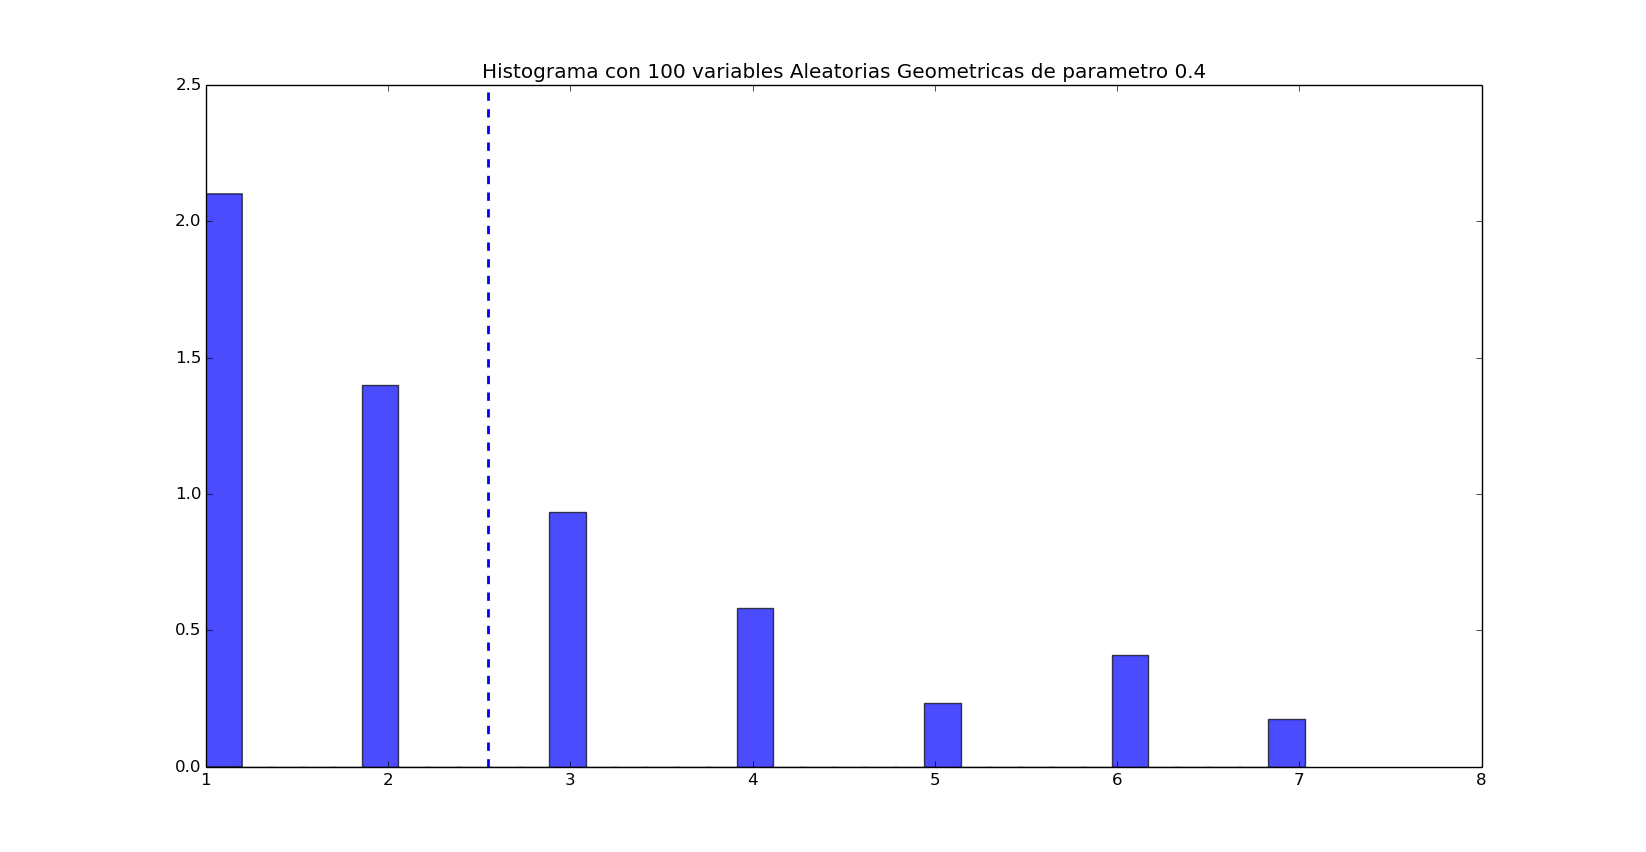
\includegraphics[scale=0.3]{100geo}}
\end{figure}


\begin{figure}[hbt]
\noindent\makebox[\textwidth]{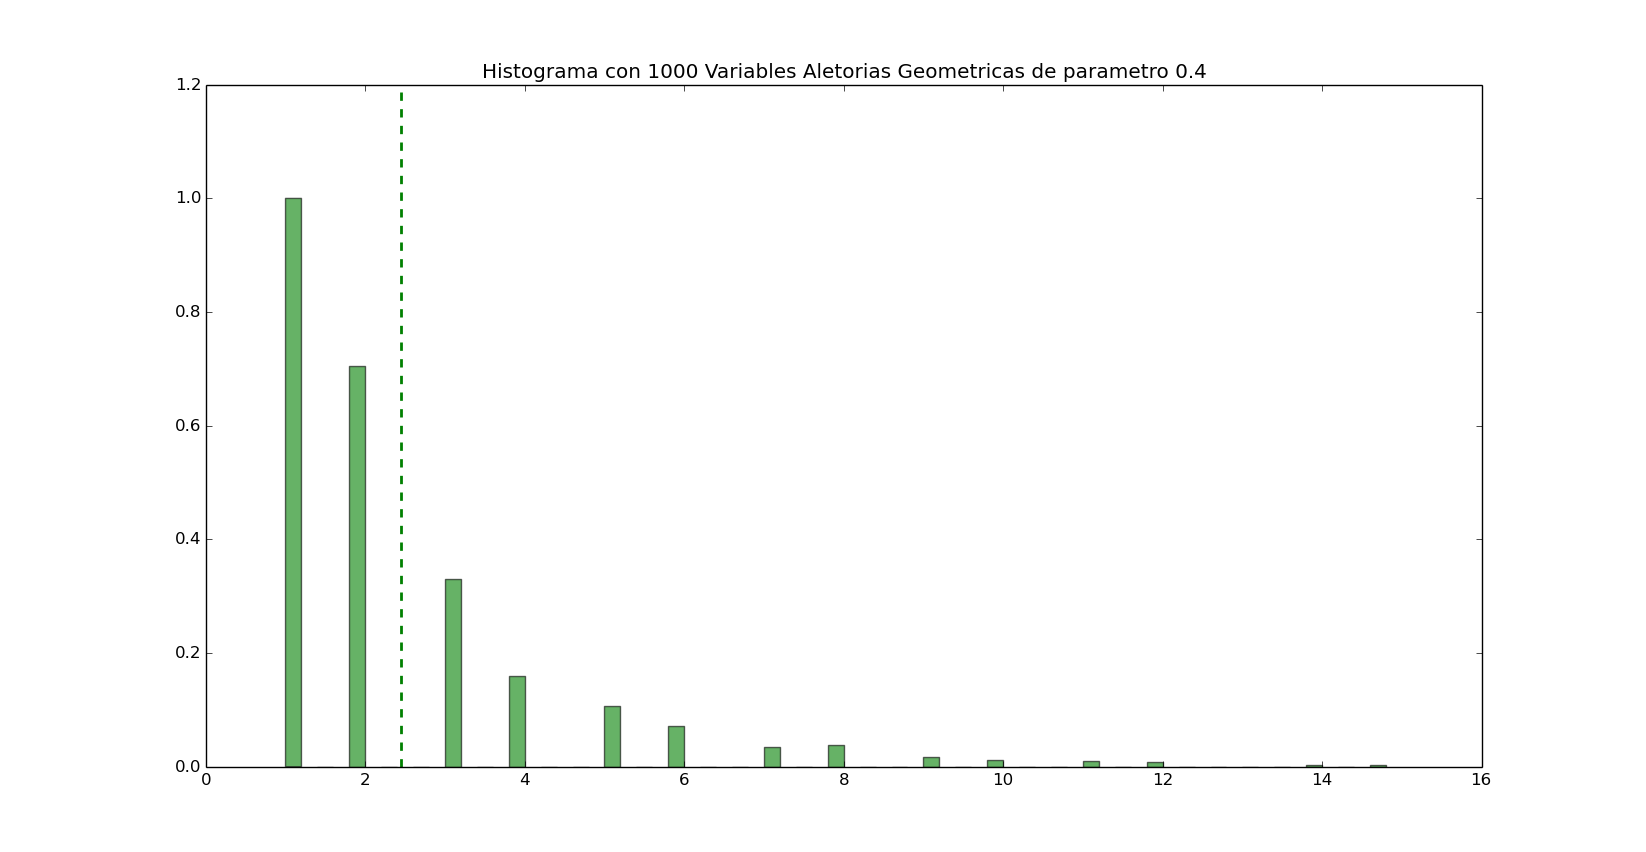
\includegraphics[scale=0.3]{1000geo}}
\end{figure}

\pagebreak

\begin{figure}[hbt]
\noindent\makebox[\textwidth]{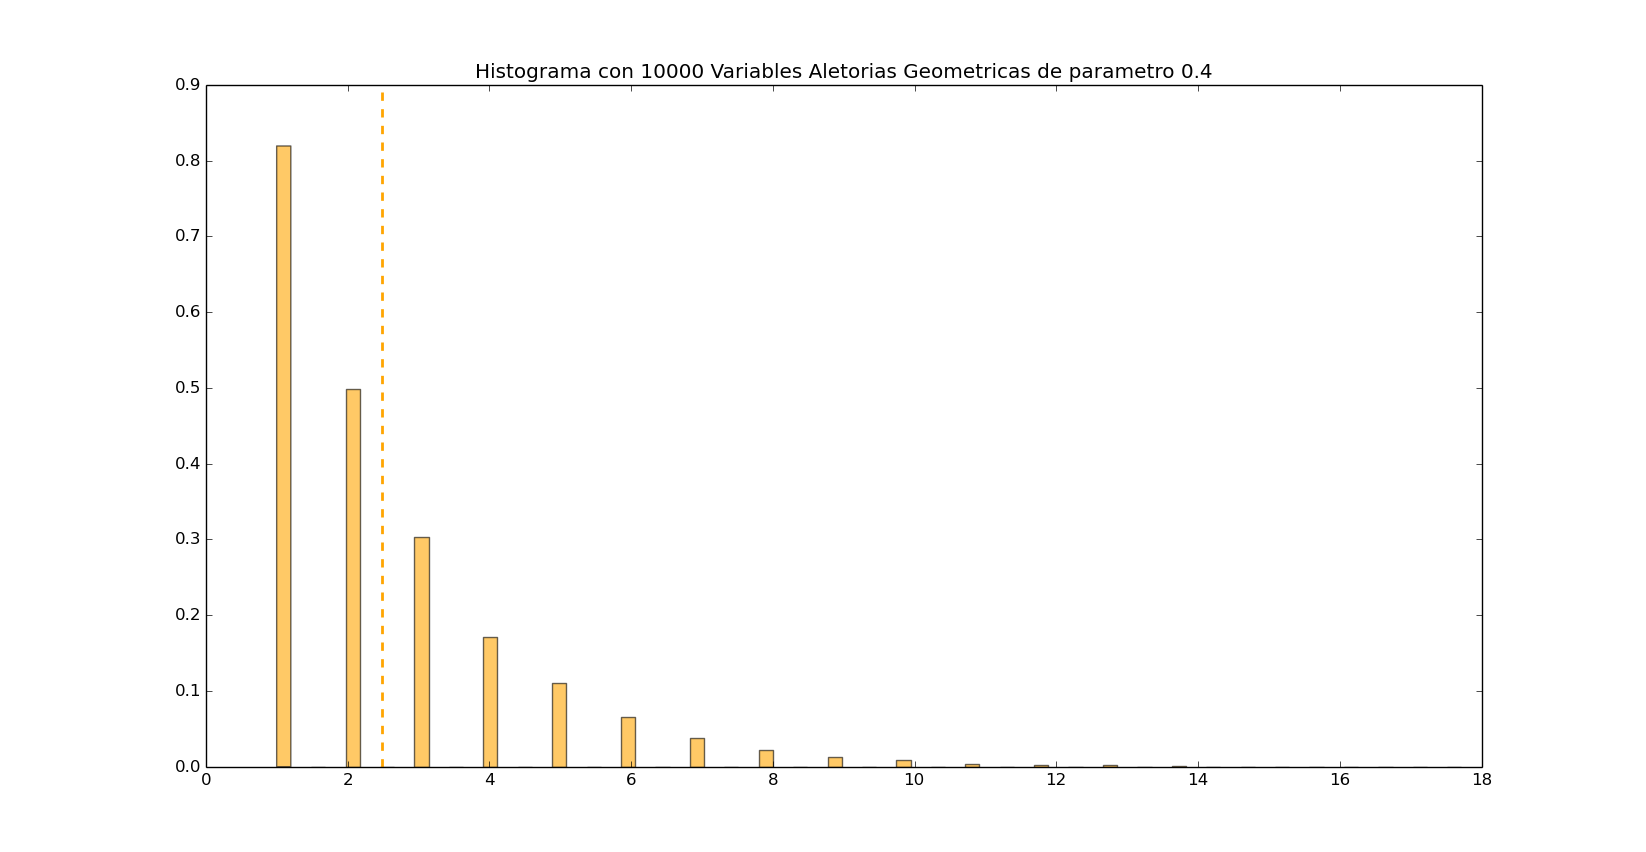
\includegraphics[scale=0.27]{10000geo}}
\end{figure}


\begin{figure}[hbt]
\noindent\makebox[\textwidth]{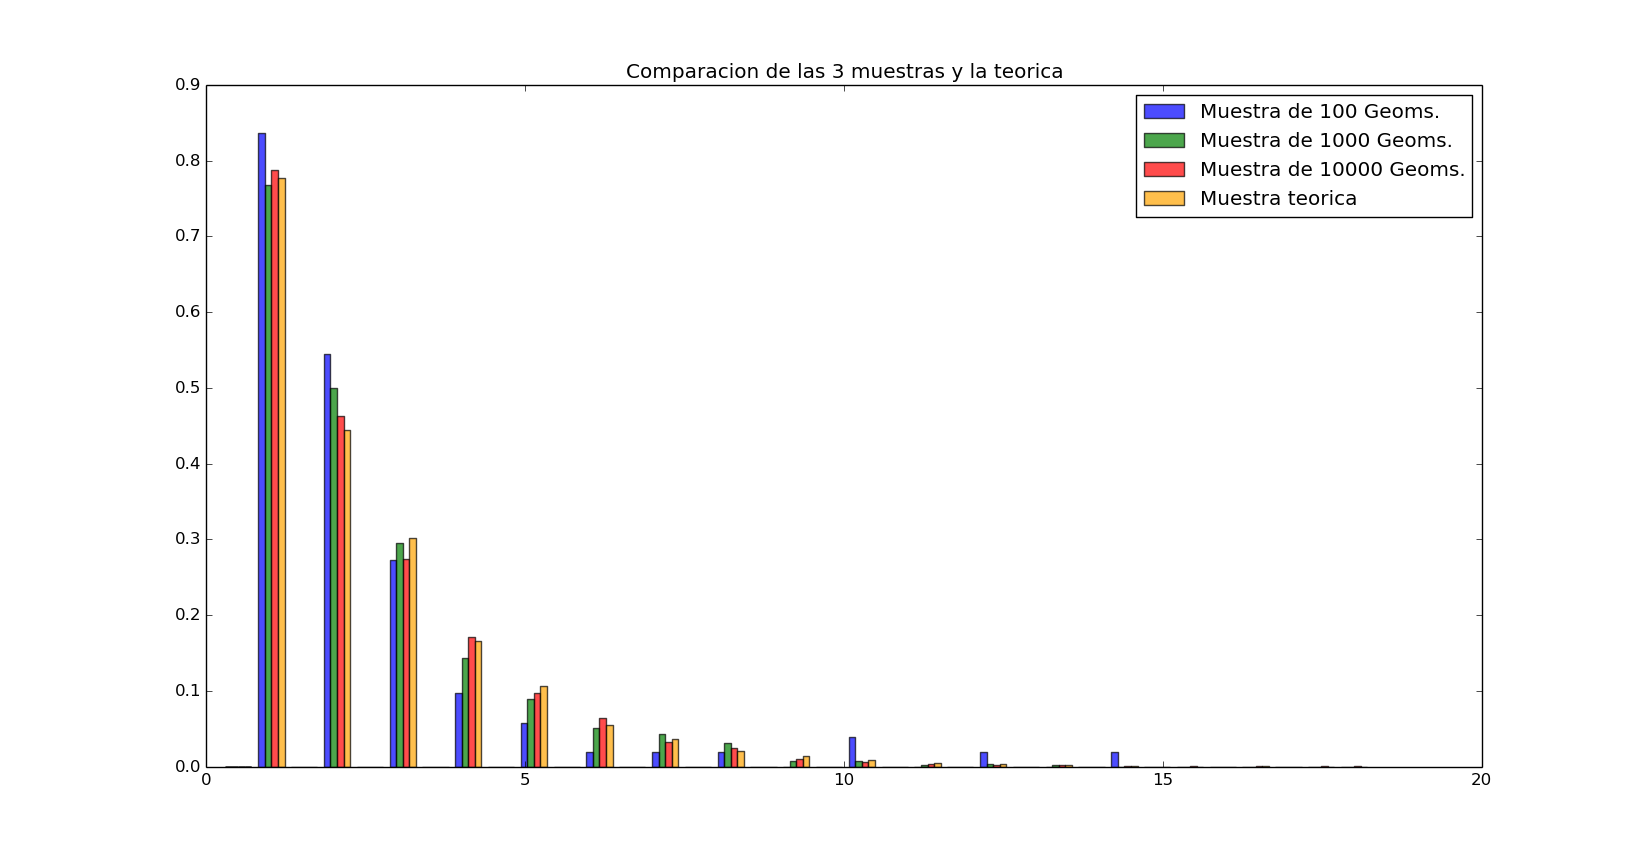
\includegraphics[scale=0.34]{teoricageo}}
\end{figure}


En vista al último histograma, podemos observar que a medida que la muestra de variables aleatorias
crece, se va acercando al límite teórico de una variable aleatoria $\mathcal{G}$(0.4).
Por lo que podríamos estar casi seguros (si no contáramos con la hipótesis que la muestra proviene
efectivamente de variables aleatorias $\mathcal{G}$(0.4)) que las observaciones tienen
dicha distribución.

\pagebreak

\section*{Test $\chi^2$}

\vspace{0.4in}

Realizaremos una estimación del p-valor a partir de la hipótesis de que la muestra está distribuida
con variable aleatorias $\mathcal{G}$(0.4).

Para esto, plantearemos dos hipótesis:

\begin{itemize}
 \item $H_0$: la muestra está distribuida con variable aleatorias $\mathcal{G}$(0.4).
 \item $H_a$: la muestra no está distribuida con variables aleatorias $\mathcal{G}$(0.4).
\end{itemize}

Definiremos el estadístico $T$ como:

\[T = \sum\limits_{i=1}^n \frac{(N_i - n p_i)^2}{n p_i}\]

donde:

\begin{itemize}
 \item $n$ es el tamaño de la muestra
 \item $N_i$ es la frecuencia observada sobre el valor $i$-ésimo.
 \item $p_i$ es la probabilidad de un valor que sea igual a $i$ (es decir, $p_i = P(X=i) = 0.4*(1 - 0.4)^i$
\end{itemize}

Entonces, tenemos que

\[p-valor \approx P\{\chi^2_{k-1} \geq t\}\]

Por lo tanto, podemos calcular $j$ estadísticos $T_1,...,T_j$
y aproximar

\[\frac{\#\{i | T_i \geq t\}}{j} \approx P\{T \geq t\}\]

Se han observado los siguientes valores:

\begin{itemize}
 \item Con $n$ = 100 Observaciones
 \subitem $t_{obs}$ = 10.9768
 \subitem $p-valor$ = 0.435
 \item Con $n$ = 1000 Observaciones
 \subitem $t_{obs}$ = 12.9523
 \subitem $p-valor$ = 0.605
 \item Con $n$ = 10000 Observaciones
 \subitem $t_{obs}$ = 20.4434
 \subitem $p-valor$ = 0.454
\end{itemize}

Como los $p-valores$ son altos ( $>$ 0.1) no tenemos suficiente evidencia para rechazar $H_0$.

\pagebreak

\section*{Modelos de ajuste de datos}

Se proponen las siguientes familias de distribuciones para el ajuste de los datos: Normal, Lognormal y Gamma.
A continuación se estimarán los parámetros por el método de máxima verosimilitud:

\subsection*{Distribución Normal}

Para los parámetros $\mu$ y $\sigma$ usaremos los siguientes estimadores:

\vspace{0.4in}

\[\bar{X} = \hat{\mu} = \sum\limits_{i=1}^n \frac{X_i}{n}\]


\[\hat{\sigma}^2 = \sum\limits_{i=1}^n \frac{(X_i - \bar{X})^2}{n}\]

\vspace{0.4in}
Las estimaciones obtenidas con tales estimadores son:
\vspace{0.4in}


$\bar{X}$ = 366.127

\vspace{0.1in}
$\hat{\sigma}^2$ = 16.41


\subsection*{Distribución Lognormal}
Para los parámetros $\mu$ y $\sigma$ usaremos los siguientes estimadores:

\vspace{0.4in}

\[\bar{X} = \hat{\mu} = \sum\limits_{i=1}^n \frac{\ln{(X_i)}}{n}\]


\[\hat{\sigma}^2 = \sum\limits_{i=1}^n \frac{(\ln{(X_i)} - \bar{X})^2}{n}\]

\vspace{0.4in}
Las estimaciones obtenidas con tales estimadores son:
\vspace{0.4in}


$\bar{X}$ = 5.902

\vspace{0.1in}
$\hat{\sigma}^2$ = 0.000123

\pagebreak


\subsection*{Distribución Gamma}
Para los parámetros $\alpha$ y $\lambda$ usaremos los siguientes estimadores (aproximación de Thom):

\vspace{0.4in}

\[A = \ln{(\bar{X})} - \sum\limits_{i=1}^n \frac{\ln{(X_i)}}{n}\]


\[\hat{\alpha} = \frac{1}{4A}\bigg(1 + \sqrt{1 + \frac{4A}{3}}\bigg)\]

\[\hat{\lambda}=\frac{\hat{\alpha}}{\bar{X}}\]
\vspace{0.4in}
Las estimaciones obtenidas con tales estimadores son:
\vspace{0.1in}


$\hat{\alpha}$ = 8139.516

\vspace{0.1in}
$\hat{\lambda}$ = 22.231


\subsection*{Calidad de los ajustes}

Ahora que tenemos valores para los estimadores de todas las distribuciones propuestas
podemos ver reflejado en un histograma qué tan bien se adaptan a nuestro modelo.

\begin{figure}[hbt]
\noindent\makebox[\textwidth]{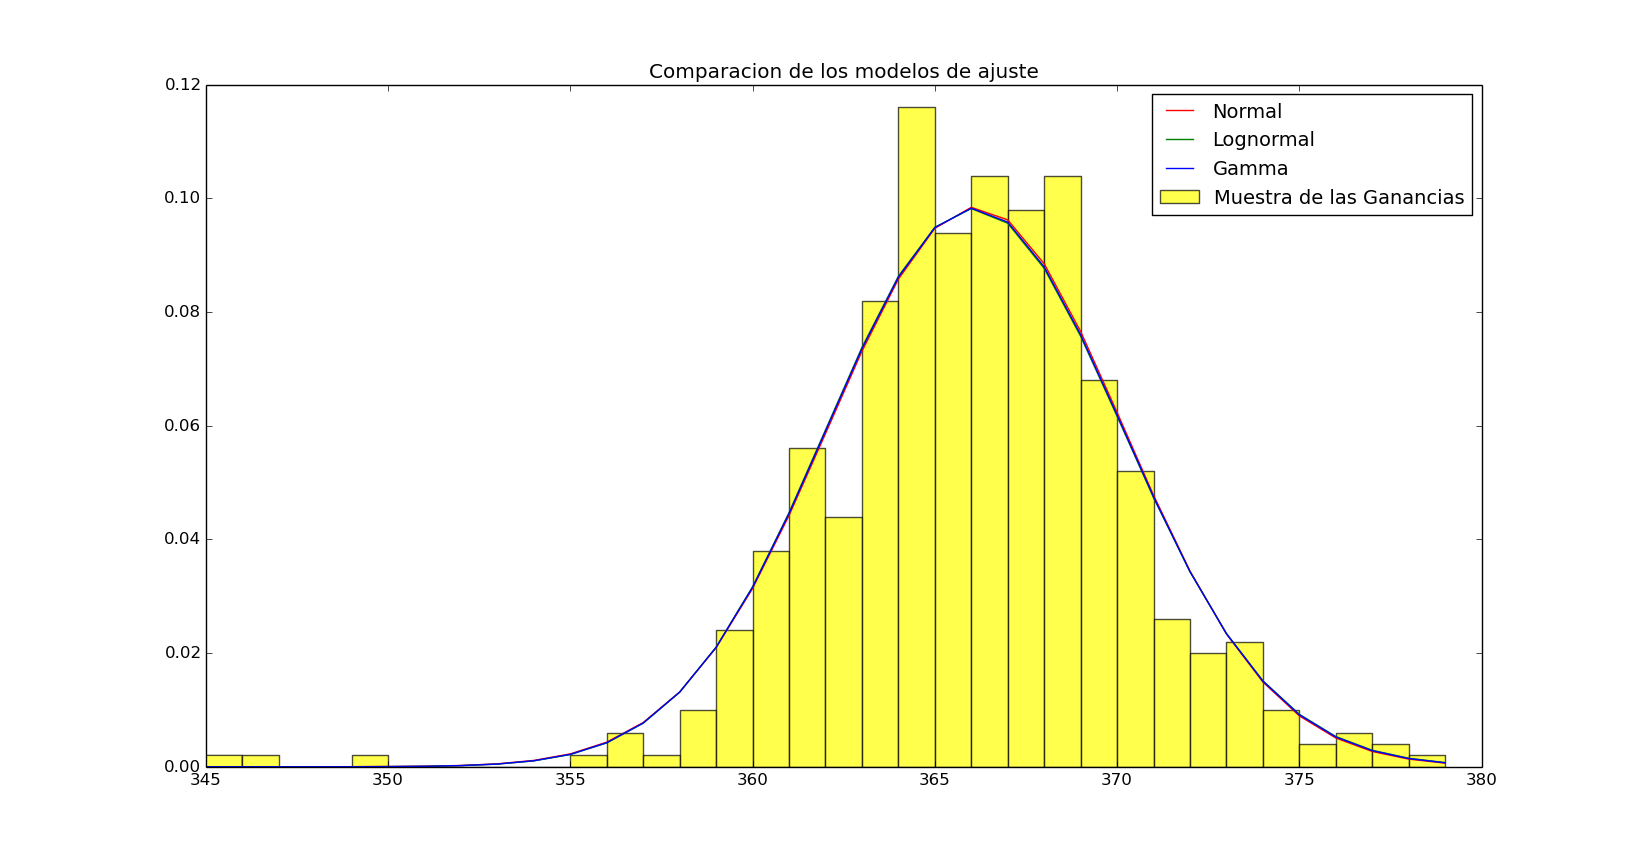
\includegraphics[scale=0.34]{modelosdeajuste}}
\end{figure}

El histograma refleja que, además que las tres distribuciones se parecen mucho, las tres se adaptan muy bien a nuestra muestra.

\pagebreak

\section*{Test de Kolmogorov-Smirnov}
\vspace{0.2in}

Para determinar cuál de las distribuciones propuestas se adapta mejor como modelos para nuestros datos, procederemos a obtener los $p-valores$ correspondientes
a cada distribución con la muestra, y eligiremos aquella que tenga el más alto.

Definamos $F_e$ como la acumulada empírica de la muestra y a $F$ como la acumulada de la distribución de la muestra bajo la hipótesis $H_0$.
Y sea el estadístico $D$ definido de la siguiente manera:

\[D \equiv \sup\limits_{-\infty < x < \infty} | F_e(x) - F(x)| \]

\[D^+ \equiv \sup\limits_{-\infty < x < \infty} \{F_e(x) - F(x)\}\]

\[D^- \equiv \sup\limits_{-\infty < x < \infty} \{F(x) - F_e(x)\}\]


\[D \equiv \textit{máx} \{D^+, D^-\} \]

Entonces, sea $d$ el estadístico observado de nuestra muestra, y sean

$D_1,...,D_j$, $j$ estadísticos, entonces aproximemos el $p-valor$ de la siguiente manera

\[\frac{\#\{i | D_i \geq d\}}{j} \approx P\{D \geq d\} = p-valor\]

Ahora que tenemos los valores de todos los estimadores de los ajustes propuestos, procedemos a calcular sus estadísticos $d$ y sus $p-valores$.

\subsection*{Ajuste Normal}

\vspace{0.2in}

$H_0:$ Los datos observados provienen de una muestra con distribución $\sim \mathcal{N}$(366.127,16.41).
\vspace{0.2in}

\noindent$H_a:$ Los datos observados no provienen de una muestra con distribución $\sim \mathcal{N}$(366.127,16.41).
\vspace{0.2in}

\noindent$\hat{\mu} =$ 366.127
\vspace{0.2in}

\noindent$\hat{\sigma^2} =$ 16.41
\vspace{0.2in}

\noindent Estadístico $d$ = 0.0416
\vspace{0.2in}

\noindent$p-valor =$ 0.3418
\vspace{0.2in}

Por lo tanto, al ser un $p-valor$ más bien alto (con que sea mayor a 0.1 alcanza, o 0.05 en otros casos), no disponemos de evidencia suficiente para
refutar $H_0$ como una hipótesis válida.


\subsection*{Ajuste Lognormal}

\vspace{0.2in}

$H_0:$ Los datos observados provienen de una muestra con distribución $\sim \mathcal{LN}$(5.902, 0.000123).
\vspace{0.2in}

\noindent$H_a:$ Los datos observados no provienen de una muestra con distribución $\sim \mathcal{LN}$(5.902,0.000123).
\vspace{0.2in}

\noindent$\hat{\mu} =$ 5.902
\vspace{0.2in}

\noindent$\hat{\sigma^2} =$ 0.000123
\vspace{0.2in}

\noindent Estadístico $d$ = 0.0433
\vspace{0.2in}

\noindent$p-valor =$ 0.2978
\vspace{0.2in}

Por lo tanto, al ser un $p-valor$ más bien alto (con que sea mayor a 0.1 alcanza, o 0.05 en otros casos), no disponemos de evidencia suficiente para
refutar $H_0$ como una hipótesis válida.


\subsection*{Ajuste Gamma}

\vspace{0.2in}

$H_0:$ Los datos observados provienen de una muestra con distribución $\sim \gamma$(8139.516,22.231).
\vspace{0.09in}

\noindent$H_a:$ Los datos observados no provienen de una muestra con distribución $\sim \mathcal{N}$(8139.516,22.231).
\vspace{0.2in}

\noindent$\hat{\alpha} =$ 8139.516
\vspace{0.2in}

\noindent$\hat{\lambda} =$ 22.231
\vspace{0.2in}

\noindent Estadístico $d$ = 0.0427
\vspace{0.2in}

\noindent$p-valor =$ 0.3122
\vspace{0.2in}

Por lo tanto, al ser un $p-valor$ más bien alto (con que sea mayor a 0.1 alcanza, o 0.05 en otros casos), no disponemos de evidencia suficiente para
refutar $H_0$ como una hipótesis válida.


La conclusión que podemos obtener al observar los $p-valores$ obtenidos es que, si no conociéramos con certeza cuál es la distribución
de la cual provienen los datos de la muestra (que es $\mathcal{G}(0.4)$), no tendríamos evidencia suficiente para refutar que los datos
pueden venir de cualquiera de estas distribuciones.

\pagebreak

\section*{Normalidad Asintótica de la Media Muestral}

Se realizó un análisis sobre 500 muestras de la ganancia semanal media
con respecto a 200 semanas a fin de comprobar su normalidad asintótica.

Para los parámetros $\mu$ y $\sigma$ usaremos los estimadores que se utilizaron en secciones previas, éstos son:

\vspace{0.4in}

\[\bar{X} = \hat{\mu} = \sum\limits_{i=1}^n \frac{X_i}{n}\]


\[\hat{\sigma}^2 = \sum\limits_{i=1}^n \frac{(X_i - \bar{X})^2}{n}\]

\vspace{0.4in}
Las estimaciones obtenidas con tales estimadores son:
\vspace{0.4in}


$\bar{X}$ = 365.656

\vspace{0.1in}
$\hat{\sigma}^2$ = 0.043

\vspace{0.1in}
Ahora que disponemos de las estimaciones puntuales, plantearemos una hipótesis nula y probaremos
mediante el test de Kolmogorov-Smirnov si podemos rechazar dicha hipótesis o si no contamos con
evidencia suficiente para refutar.


Entonces, sean:
\vspace{0.2in}

\noindent$H_0:$ Los datos observados provienen de una muestra con distribución $\sim \mathcal{N}$(365.656,0.043).
\vspace{0.11in}

\noindent$H_a:$ Los datos observados no provienen de una muestra con distribución $\sim \mathcal{N}$(365.656,0.043).
\vspace{0.2in}


El test de Kolmogorov-Smirnov nos muestra los siguientes resultados:

\vspace{0.2in}

\noindent Estadístico $d$ = 0.021087
\vspace{0.2in}

\noindent$p-valor =$ 0.9793
\vspace{0.2in}

Por lo tanto, al ser un $p-valor$ más bien alto (con que sea mayor a 0.1 alcanza, o 0.05 en otros casos), no disponemos de evidencia suficiente para
refutar $H_0$ como una hipótesis válida.

\pagebreak

\section*{Conclusión}

De mano de la inferencia estadística, la bondad de ajuste y una muestra de datos que fueron generados a partir de
una variable $\sim \mathcal{G}(0.4)$, hemos sido capaces de determinar que las ganancias semanales responden de manera
correcta a una distribución $\mathcal{N}(366.127,16.41)$.

También fuimos capaces de realizar tests para demostrar que la ganancia media es asintóticamente $\sim \mathcal{N}$(365.656,0.043).

Son resultados realmente soprendentes, pero no más que la teoría que los respalda.
\end{document}
